
\documentclass[sigconf, nonacm=true]{acmart}
\setcopyright{none}
%\documentclass[9pt,twocolumn]{extarticle}
%\usepackage[a4paper,margin=0.8in]{geometry}
%\usepackage{dblfloatfix}
%\usepackage{graphicx}
\usepackage{tabularx}
%\usepackage[T1]{fontenc}
%\usepackage{tgschola}

\begin{document}
\title{ECOLM Futures Review}

\author{Chris Cannam}
\orcid{https://orcid.org/0009-0001-9814-6512}
\affiliation{%
  \institution{Particular Programs Ltd}
  \city{London}
  \country{UK}}
\email{chris.cannam@particularprograms.co.uk}

\author{David Lewis}
\affiliation{%
  \institution{Goldsmiths, University of London}
  \city{London}
  \country{UK}}
\email{d.lewis@gold.ac.uk}

\author{Tim Crawford}
\affiliation{%
  \institution{Goldsmiths, University of London}
  \city{London}
  \country{UK}}
\email{t.crawford@gold.ac.uk}

\maketitle
\begin{sloppypar}
  
  \section{Background and Motivation}

  \subsection{What is ECOLM?}

  ECOLM\footnote{http://igor.gold.ac.uk/isms/ecolm/} or ``Electronic
  Corpus of Lute Music'' was a series of research projects aiming to
  develop a queryable online database of lute tablature encodings, of
  quality suitable for scholarly use.

  Two critical, and still relevant, goals were:
  
  \begin{enumerate}
  \item To store and deliver encodings of music, not only metadata;
  \item To be trustworthy for scholarly use: for example, sources are
    identified, reliability of attribution is noted, editorial changes
    are pointed out, and the schema distinguishes between performance
    and diplomatic transcriptions.
  \end{enumerate}
  
  Here we use the name ECOLM broadly to refer to this design of
  database application, as well as to the past research projects of
  that name and to the existing
  system\footnote{http://doc.gold.ac.uk/isms/ecolm/database/} that
  they produced.

  \subsection{Aim and Structure of this Review}

  We aim to review the premise and outcomes of ECOLM and to consider
  whether a ``lightweight path to sustainability'' can be found that
  can be incrementally extended to other tablature resources.

  In section \ref{enumerate-resources} we first set out the history of
  ECOLM and enumerate other resources of interest. Section
  \ref{user-context} identifies some typical users of such resources
  and describes our findings from user interviews. In section
  \ref{technical} we outline the technical makeup of each of these
  resources and some related sites of interest. Section
  \ref{desirable-qualities} summarises the desirable qualities we seek
  in a solution, and section \ref{future} suggests three possible
  future courses of action.

  \section{ECOLM and Other Resources}\label{enumerate-resources}
  
  \subsection{The ECOLM Projects}

  %%%!!! + bibliography
  %%%!!! + URLs in footnote
  \begin{itemize}
  \item {\bf ECOLM} (1999-2002) was a project run by Tim Crawford,
    initially at King's College London, which produced a queryable
    database of lute encodings with metadata with a web interface. The
    resulting service is still accessible today through a
    public-facing server hosted at Goldsmiths.
  \item {\bf ECOLM II} (2002-2006) was a successor project which
    expanded the ECOLM database and used it for some computational
    musicological investigations.
  \item {\bf ECOLM III} (2012) was a short project with the goal of
    adding further high-quality encodings by crowd-sourcing
    corrections of OMR (optical music recognition) scans.
    %%%!!! say more about this later
  \end{itemize}

  The ECOLM database as available online contains about 2,000
  tablature encodings, manually curated, of relatively high quality
  with accompanying metadata.

  \subsection{Other Lute Tablature Resources}

  Several other collections of lute music have been collected and
  placed online by various curators. Of particular interest are:
  \begin{itemize}
    \item {\bf Mss.slweiss.de}\footnote{https://mss.slweiss.de/}
      curated by Peter Steur and the late Markus Lutz. A metadata
      catalogue of around 68,000 listings of which the majority have
      incipits (opening ideas) encoded.
    \item {\bf Lutemusic.org}\footnote{https://lutemusic.org/} curated
      by Sarge Gerbode. Around 20,000 encodings in playing editions
      with semi-structured metadata, informally curated with limited
      version tracking or editorial notes.
    \item {\bf Lute Society publications} curated by John
      Robinson. Scans from printed periodicals intended for players,
      containing around 7,000 encodings consisting of printed music,
      prose commentary, and semi-structured metadata.
    \item {\bf Phal\`ese} curated by Jan Burgers. Around 1,000
      encodings transcribed from editions of 16th-century publisher
      Pierre Phal\`ese with publication metadata.

      %%!!! tabulate their type, content, whether published already,
      %% licence terms, how widely used
  \end{itemize}

  There are concerns about the ongoing sustainability of many of
  these, similar to those about ECOLM: curation and maintenance by
  individuals or small groups of enthusiasts, in some cases of
  retirement age; maintenance in limited periods of spare time,
  perhaps following initial short-term funding; data management using
  ad-hoc methods or private systems that are not accessible to
  third-party reproduction; lack of data export facilities or support
  for common interchange formats.

  Therefore, we would prefer to find a solution with the potential to
  incorporate and maintain data from these resources as well.

  The lutemusic.org transcriptions are explicitly Creative Commons
  NC-SA licensed, and the maintainers of the other listed resources
  have indicated willingness to contribute to a potential combined
  dataset.
  
  \renewcommand{\arraystretch}{1.2}
  \setlength{\tabcolsep}{4pt}
  
  \begin{table*}[t]
  \caption{Status of data and metadata in online lute tablature resources}
  \small
      \begin{tabularx}{\textwidth}{|l|X|X|X|X|X|X|X|X|X|}
        \hline
        & \multicolumn{4}{|c|}{\bf Data} & \multicolumn{5}{|c|}{\bf Metadata} \\
        \hline
        & Encoded tablature & OTR scanned pages & Facsimile images & Published PDFs
        & Works linked to encodings & Ordered work-lists & Textual commentary & Textual references to models & Structured metadata \\
        \hline
            {ECOLM I/II} & Yes & Partial & Yes & & Yes & Yes & & Partial & Yes \\
        \hline
            {Mss.slweiss.de} & Yes & & & & & Yes & & & Partial \\
        \hline
            {Lutemusic.org} & Yes & & Partial & Yes & Partial & & & & Partial \\
        \hline
            {Lute Society} & Yes &  & & Yes & & Yes & Yes & Yes & \\
        \hline
            {Phal\`ese} & Yes & & & Yes & Partial & Partial & Yes & Yes & \\
            \hline
      \end{tabularx}
  \label{table:datasets}
  \end{table*}
  
  %%!!! include section about other non-lute resources: RISM being the
  %%!!! most obvious but also anything else anyone else mentioned
  
  \section{Understanding User Context}\label{user-context}

  The resources we are considering serve a spectrum of audiences. At
  one end, lutemusic.org aims at performers and includes edited
  transcriptions with relatively little scholarly metadata or
  editorial comment. At the other, ECOLM was aimed at computational
  musicologists and prioritises diplomatic facsimiles and
  transcriptions that preserve original scribal idiosyncracies.

  In this review we are particularly concerned with sustainability for
  musicology and other academic purposes. To this end, we conducted
  informal interviews with three exemplary users of online early-music
  resources, in order to understand scholarly expectations. These were
  a ``traditional'' musicologist, a computational musicologist, and a
  lute performer and teacher.
  
  \subsection{Musicologist}

  Depending on the material they are looking for, the musicologist we
  spoke to may begin by searching the
  RISM\footnote{https://rism.info/} or
  Cantus\footnote{https://cantus.uwaterloo.ca/} databases. They
  routinely start with a search by composer or source, because titles
  tend to have too many historical variants.

  They find diplomatic transcriptions (i.e. closely following the
  source without editorial intervention) the most useful, but are
  grateful to find any transcription. However, they always refer to
  the facsimile as well, regardless of the status of any
  transcriptions, so can often do without editorial notes.
  
  This musicologist was particularly interested in dual tablature and
  staff renderings, because they are not a specialist in
  tablature. They would also appreciate the opportunity to annotate or
  correct unreliable transcriptions for their own use.
  
  \subsection{Computational Musicologist}

  The computational musicologist we spoke to would typically also
  begin by searching RISM. They trust that metadata in RISM is more
  authoritative than elsewhere.
  
  They consider trust very important, and appreciate annotations about
  the original source, transcriber, and editorial interventions. They
  can work with unreliable transcriptions, if their quality is known
  and original sources are properly described.
  
  When considering the user interface to a dataset, they appreciate a
  simple presentation and single search function as their first entry
  point. They described the ability to refine results via facets as
  more useful than the ability to construct complex queries from the
  outset.
  
  The computational musicologist expects the ability to download
  results (up to possibly the whole dataset) or to query data via API,
  for use with computational tools such as music21 or Humdrum locally.
  
  \subsection{Lute Performer and Teacher}

  The lute performer and teacher we spoke to would often begin by
  using the most informal performance resources, simply because they
  have the most material available. This causes problems
  cross-referencing with more authoritative material. They find
  information about the original source, transcriber, and editorial
  interventions extremely important, but these are often lacking in
  performance resources.
  
  As a teacher, they expect students to know the history of the
  editions they use when performing. They would greatly appreciate
  something containing modern performing editions, as at
  lutemusic.org, but with more reliable editorial commentary.
      
  In the absence of trustworthy editorial information, they
  effectively need to compare every note with the facsimile before
  making serious use of a transcription.

  \subsection{Common Threads}

  Trust and provenance are common themes in discussion with all three
  of our exemplary users. They have different requirements for
  content, format, detail of editorial notes and so on, but share a
  desire to know the quality of transcription and level of editorial
  intervention they are dealing with.

  There was also some consensus about the value of simple search with
  subsequent refinement, of a cleanly-designed results layout
  including inline incipits, and of API and data provision.
  
  The musicological specialists were comfortable with RISM and would
  prefer some level of compatibility, perhaps as far as having the
  works indexed from RISM and metadata managed there.

  None of the three indicated they would hope to {\em contribute}
  material to a dataset like this, although they might appreciate the
  ability to make corrections.

  The users mentioned some other sites which they regarded as
  particularly useful or as good examples to learn from. These are
  listed in section \ref{other-sites} below.
  
  \section{Technical Review}\label{technical}

  We studied the technical makeup of each of these resources and of
  other sites of interest, including retrieving data and schema dumps
  and mapping the schema where applicable. Schema diagrams and
  accompanying notes are included separately at the end of this
  document.
  
  \subsection{Tablature Resources}
  
  \subsubsection{ECOLM}

  ECOLM is a web application written in PHP backed by an SQL
  database.

  Entity relationships are modelled directly in the schema rather than
  as literal relations in the RDF or triple-store sense. Relations are
  hardcoded and cannot be changed once the database has been loaded.
  
  A concept known as ``clusters'' is used to give some support for
  more general relations within the schema. The most common use is for
  grouping a number of ``pieces'' (representations within published
  sources) into a ``work'' (a single musical composition).

  The schema supports modelling of confidence levels for relations,
  and dates are modelled with a custom type that supports
  partially-bounded queries and queries of varying precision.
  
  The same database is used for administrative work (user logins and
  editorial control) as for content records; there is an expectation
  that data entry and management are carried out within the same ECOLM
  application as query and retrieval.

  Transcriptions are stored in TabCode, a format devised for the
  purpose and not widely used elsewhere. Converters between TabCode
  and other formats are readily available.
 
  The degree of rigour in organisation means that, while it may be
  tricky to convert or adapt to another format or system, such an
  effort will probably succeed without too many loose ends.

  See section \ref{ecolm-data} for more technical details and a schema
  diagram.

  \subsubsection{mss.slweiss.de}

  This is a web application written in PHP and driven entirely from
  CSV-like files with a semicolon-separated tabular format.
  
  There is a flat directory containing one CSV-like file per source.
  Separate index files in the same CSV-like format contain manuscript
  metadata and concordances.

  Incipits are embedded in the CSV files, in ABC format, and rendered
  to SVG from the PHP scripts to be served to the browser. Query
  capabilities are limited and full transcriptions are not included.

  The dataset has been version-controlled since 2013, and is
  well-organised and looks relatively easy to deal with.
  
  \subsubsection{lutemusic.org}

  This is implemented by directly exposing a static file hierarchy
  through a web server.
  
  The site uses a hierarchical organisation, with separate filesystem
  trees by composer, source, and facsimile. Composer and source trees
  contain Fronimo tab transcriptions with derived MIDI and PDF
  renderings.
  
  The facsimile tree contains images (typically PNG) closely cropped
  with thresholding, apparently intended for clear reading from screen
  rather than as historical page facsimiles.
    
  A separate, apparently older, tab hierarchy also present with
  tab-format files.
  
  The files are indexed using a hand-maintained spreadsheet which
  contains metadata and the Fronimo file index. There does not appear
  to be versioning for files or the index.
  
  This design is attractively simple, but its irregular organisation
  may make adaptation relatively high risk.
    
  \subsubsection{Lute Society}

  This consists of facsimiles and transcriptions from the Lute News
  paper publication, organised by issue number.
  
  The organisation is on filesystem, with PDFs and transcriptions of
  both text and tablature.
  
  There is a simple front-end available, provided by Tim
  Crawford\footnote{https://doc.gold.ac.uk/~mas01tc/jhr\_web/} which
  provides a web index via Javascript requests on the client side.
  
  The content seems well organised. The difficulty is the wide variety
  of types of material present (including a lot of prose commentary)
  and the original linear organisation intended for readers and players.
  
  \subsubsection{Phal\`ese}

  We have relatively little technical information about the Phal\`ese
  dataset. It is understood to contain transcriptions in Tab format,
  along with EPS and JPEG facsimiles and documentation mapping the
  pieces to the original volume and location.

  \subsection{Other Sites of Interest}\label{other-sites}
  
  \subsubsection{RISM}

  RISM\footnote{https://rism.info/} (R\'epertoire International des
  Sources Musicales) is a catalogue of musical sources. It ``documents
  what exists and where it is
  kept''\footnote{https://opac.rism.info/main-menu-/kachelmenu/about}. That
  is, it is not a library but an index of libraries and the sources
  they contain. It has a historical focus on physical sources rather
  than abstract works (although this may be changing) and although
  some records have incipits attached, it does not otherwise serve
  musical content.

  As we saw in section \ref{user-context}, musicologists routinely
  expect sources to be indexed in RISM and may expect it to offer the
  most authoritative source metadata.

  The RISM project also publishes a web application for entry and
  management of musical source catalogue data, called Muscat. See
  section \ref{muscat-data} for details about the schema used by
  Muscat.

  RISM records are stored in MARC\footnote{https://www.loc.gov/marc/}
  (Machine Readable Cataloging) format and are available as MARC or
  RDF data via API.

  \subsubsection{DIAMM}

  DIAMM\footnote{https://www.diamm.ac.uk/} (Digital Image Archive of
  Medieval Music) is an archive of scanned manuscripts, mainly from
  before 1600. It also indexes sources whose images are stored
  elsewhere. Images are typically of high quality with accompanying
  metadata describing the physical artifact in some detail.

  DIAMM has an API providing metadata in a JSON encoding, though
  apparently not RDF or JSON-LD.
  
  \subsubsection{Vihuela Database}

  The Vihuela Database\footnote{https://vihuelagriffiths.com/} of John
  Griffiths is a research-focused index of vihuela music and
  information about the vihuela. It includes a browseable and
  searchable list of pieces with incipits in image form and some text
  commentary. Significant fantasia themes are indexed separately by
  melody. The site does not appear to offer an API or data linking.

  Our consulted lute performer/teacher praised this site for its clear
  presentation of search results with inline incipits (figure
  \ref{fig:vihuela}) and use of editorial commentary.
  
  \begin{figure}[h]
  \centering
  \caption{Vihuela Database search results example}
  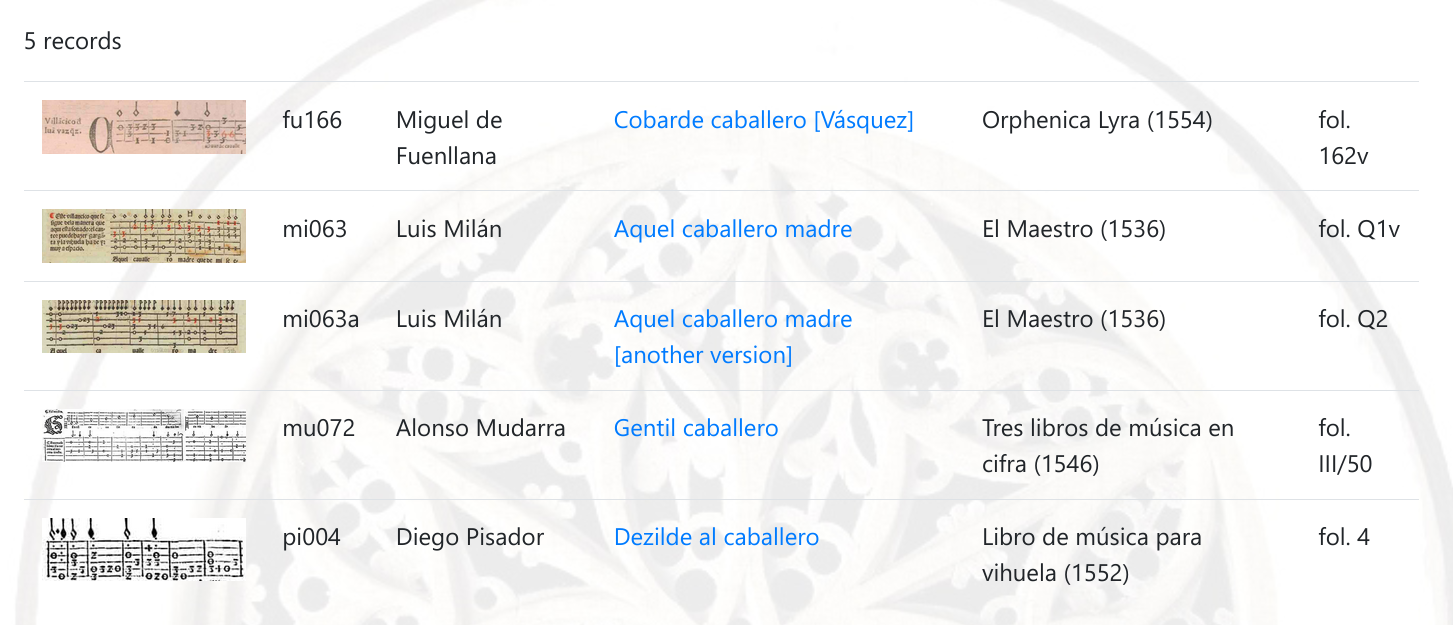
\includegraphics[width=\columnwidth]{images/vihuela-search-results}
  \label{fig:vihuela}
  \end{figure}
  
  \subsubsection{Josquin Research Project}

  The Josquin Research Project\footnote{https://josquin.stanford.edu/}
  from Jesse Rodin and Craig Sapp at Stanford is an index of early
  polyphonic music with full digitised scores. It is driven from a
  transparent catalogue of Humdrum-format scores, maintained under
  version control in a Git repository with a submodule per composer
  and available from the website in-page or via an API.

  Our consulted computational musicologist praised this site for its
  straightforward search interface, presentation of results including
  useful details such as vocal range plots, and publication of raw
  data for computational use.
  
%  \subsubsection{earlymusicsources.com}
%  \subsubsection{earlymusiconline.org}
  \subsubsection{IMSLP / Petrucci}

  IMSLP (the International Music Score Library Project or Petrucci
  Music Library) is a very widely used crowd-sourced library of
  public-domain and Creative Commons licensed sheet music. Managed
  using MediaWiki, it makes a priority of encouraging community
  contributions over authoritative editorial review. Works are often
  available in multiple versions including scans and transcriptions,
  typically rendered as PDFs rather than in machine-readable
  form. Depending on the composition, works may feature in full score,
  parts, and arrangements, and tablature often appears where
  applicable. There is some linkage to other informal resources such
  as Wikipedia as well as to formal authorities such as VIAF.
  
  \section{Desirable Qualities of a Solution}\label{desirable-qualities}
  \subsection{Social}

  We see three requirements for a socially sustainable outcome:

  \begin{enumerate}
  \item Sufficient immediate utility to our audience(s) to justify our
    work and to ensure that users are invested in the outcome;
  \item Sufficient scholarly quality to ensure that the outcome is
    genuinely helpful in expanding and improving the work that our
    users are able to do;
  \item Sufficiently accessible and robust technical choices to enable
    other enthusiast users to maintain and contribute to the outcome
    without substantial difficulty or risk of causing damage.
  \end{enumerate}

  Bluntly, we need to (1) hook users, (2) genuinely help them to do
  their best work, and (3) make it possible for the keenest
  technically-minded ones to pick up where we left off.
  
  Points (1) and (2) were touched on several times in our interviews
  with exemplary users outlined in section \ref{user-context}. Their
  remarks about simple and accessible search functions, clear
  presentation of results with incipits, integration with RISM, and
  the habit of using the largest available dataset are all examples of
  point (1). Their remarks about trust, provenance, editorial quality
  and history, and availability of data through an API are examples of
  (2). Their references to other sites and datasets they refer to span
  both.

  For point (3) we can look to past examples from the same field and
  elsewhere. Two obvious types of ongoing contribution are
  crowd-sourcing (contributing to the existing artifact) and
  mirror/fork replication (producing another artifact based on the
  first).

  There are of course many successful crowd-sourced projects, although
  success in encouraging contributions in content can lead to even
  more difficulty in sustainable hosting or maintenance. The ECOLM III
  project attempted to crowd-source corrections for optical musical
  recognition output, with limited success, perhaps because
  contributors did not immediately get to use the fruits of their
  labour. Some other lute tablature resources employ old-school
  informal crowd-sourcing (simply encouraging people to send
  contributions to a human maintainer) with arguably more success.

  Supporting replication via mirroring or forking is a separate issue
  from crowd-sourcing and is arguably essential for a system of this
  type nowadays. It calls for publication of source code and data,
  replicable scripted testing and data population, versioning and the
  ability to merge dataset updates, and ideally a system for
  generating identifiers that is stable across instances. Some of
  these matters will be touched on in the technical requirements
  below.
  
  \subsection{Technical}

  We have divided technical qualities into required (inadvisable to
  ignore when choosing an approach) and desired.
  
  \subsubsection{Required}
  
  \begin{itemize}
  \item Use of standard formats where they exist.
    \begin{itemize}
      \item For example, existing resources store tablature and score
        incipits in a variety of formats including TabCode, ABC,
        Humdrum, or Plaine \& Easie Code, but the world is
        standardising on MEI and all of these formats can be converted
        to it, so it makes sense to use it as a presentation format in
        general.
    \end{itemize}        
  \item Provision of data through an API.
  \item Ability to absorb further upstream changes after first import,
    for adaptations of datasets that are being maintained elsewhere.
    \begin{itemize}
    \item May call for ``idempotent'', testable, automatically tested
      format conversion and import processes.
    \end{itemize}
  \item Stable identifiers for works, sources, transcriptions.
    \begin{itemize}
    \item To allow to disambiguate works and sources that appear among
      multiple input datasets.
    \item To allow transcriptions to be referred to by computational
      musicology processes, such as similarity calculations.
    \item Identifiers linked to those used in other sources, online or
      offline (particularly RISM where available).
    \end{itemize}
  \item Ability to handle substantial textual and other unstructured
    data including diagrams and multimedia.
  \end{itemize}

  \subsubsection{Desired}
  
  \begin{itemize}
  \item An ``immutable pipeline'' allowing a rebuild at any time from
    source formats that are friendly for humans to work with.
    \begin{itemize}
      \item But note the formats that other maintainers actually deem
        friendly and choose to use---these tend to be CSV and XLS, not
        ``industry'' formats like JSON or ``academic'' like RDF/Turtle.
    \end{itemize}
  \item Ready support for version-controlled updates.
  \item Ability to provide alternative front-ends over the same dataset.
  \item Support for multiple types of facsimile as well as potentially
    of transcription---for example if a source has both
    screen-optimised PNG and a detailed scan with limited editing, it
    would be useful to retain both, with suitable metadata.
  \item RISM indexing compatibility.
  \item API able to serve RDF and/or JSON-LD.
  \end{itemize}
  
  \section{Possible Paths}\label{future}

  We propose three alternative directions for sustainable development,
  as follows.
  
  \subsection{``Enhanced ECOLM''}

  In this alternative, we would retain the relational data schema of
  the existing ECOLM, which is the only one of the datasets under
  consideration to have a formal schema, and provide ETL (extract,
  transform, load) data loaders for other sources. We then publish the
  schema, data dumps, and automation to rebuild or mirror the data,
  along with the code of our query interface and encourage others to
  attach their own interfaces or tools to it.

  Advantages of this approach include the ability to preserve existing
  code and to use original ECOLM records as a reference. The existing
  schema is detailed and fairly effective, provides appropriate
  structure, and reflects some good domain-specific
  decisions. Relational data import is a well understood field, and we
  could focus on user interfaces and data conversion rather than any
  novelty of data representation. If the work fails, the result should
  be at minimum a more open publication of the existing ECOLM.

  Disadvantages include that the schema has little in common with any
  of the ad-hoc solutions other maintainers have settled on, so all
  import and export would be custom. It also has little in common with
  wider current practice. The schema is perhaps already overspecified
  for its current use, yet does not address any problems relating to
  stable identifiers, versioning, or providing queryable APIs or data
  sources.

  Although we could at least initially reuse the existing user
  interface, it is no longer considered a strength of ECOLM and would
  need some work to update to modern expectations.

  \subsection{Graph-based}

  In this alternative, we would take the fundamental representation to
  be a graph of triples in the model of RDF, and convert all metadata
  to that for import and from it for query. External data such as
  transcriptions and multimedia resources are identified by
  graph-relatable identifiers such as URIs.

  Advantages include the use of a widely-understood and accepted model
  that meets common expectations about data compatibility and API
  provision. For schema we can draw ontologies from existing systems
  including the widely-used RISM. The structure is reasonably amenable
  to versioning and to use of ``idempotent'' import flows with
  automated testing, offering the option of ongoing import of changes
  in upstream sources. In principle existing tools may be used for
  review, query, inferencing, and conversion. The use of standard
  formats with automated tests could lead to a result far more easily
  maintained or mirrored by third parties.

  The approach has difficulties as well. It discards the existing user
  interface work and requires even the existing ECOLM data to be
  converted. Although graph representations have wide application,
  they are not generally used for manual data management and therefore
  have as little in common with the ad-hoc schemas of enthusiast lute
  resources as with that of ECOLM. Significant work would be required
  to maintain stable identifier mappings from external sources. With a
  more flexible structure than ECOLM's relational database, care and
  good automated testing would be needed to avoid ``silently missing
  data'' problems on query. Finally a separate solution would be
  needed to the problem of identifying and retrieving non-graph data
  such as media resources.

  Although in this approach we could no longer use the existing ECOLM
  user interface, that may be slightly mitigated by the ability to
  adapt other graph-driven UIs to the model.

  \subsection{``RISM-aligned''}

  In this alternative, we would concentrate on compatibility with
  formats and software used by RISM. The motivating principle is that
  RISM is the dominant ``entry point'' in this field and, although our
  sources are not all up to the standard indexed by RISM, we want to
  facilitate linkage for those that are, and to be prepared if in the
  future RISM should grow to cover the whole area of directly
  represented lute tablature. The ideal future here would involve
  replacing this project entirely with an aspect of RISM.

  In this approach the metadata representation might be MARC, as it is
  within RISM, and possibly the RISM Muscat application might be used
  for management.

  \subsection{Summary of Paths}

  The three alternatives we have listed broadly correspond to common
  patterns in work of this type:

  \begin{enumerate}
  \item Choose one of the existing technical solutions already in use,
    and adapt the others to it;
  \item Adopt a higher-level ``linked data'' approach in which all
    existing resources are promoted to an interoperable format;
  \item Find an industry partner, adopt their tools, and contribute to
    their existing ecosystem.
  \end{enumerate}

  In this case RISM is the closest thing available to a
  standard-setting source of industrial tooling and integration, so it
  may serve as the equivalent of an industry partner. Hybrid
  approaches may also be practical, such as adapting the existing
  sources into a graph representation as a lowest-common-denominator
  precursor to conversion into other formats.
  
  \clearpage

  \section{Data representation in existing systems}
  
  \subsection{ECOLM II}\label{ecolm-data}
  
  \begin{figure*}[b]
  \centering
  \caption{ECOLM II database schema (record tables)}
  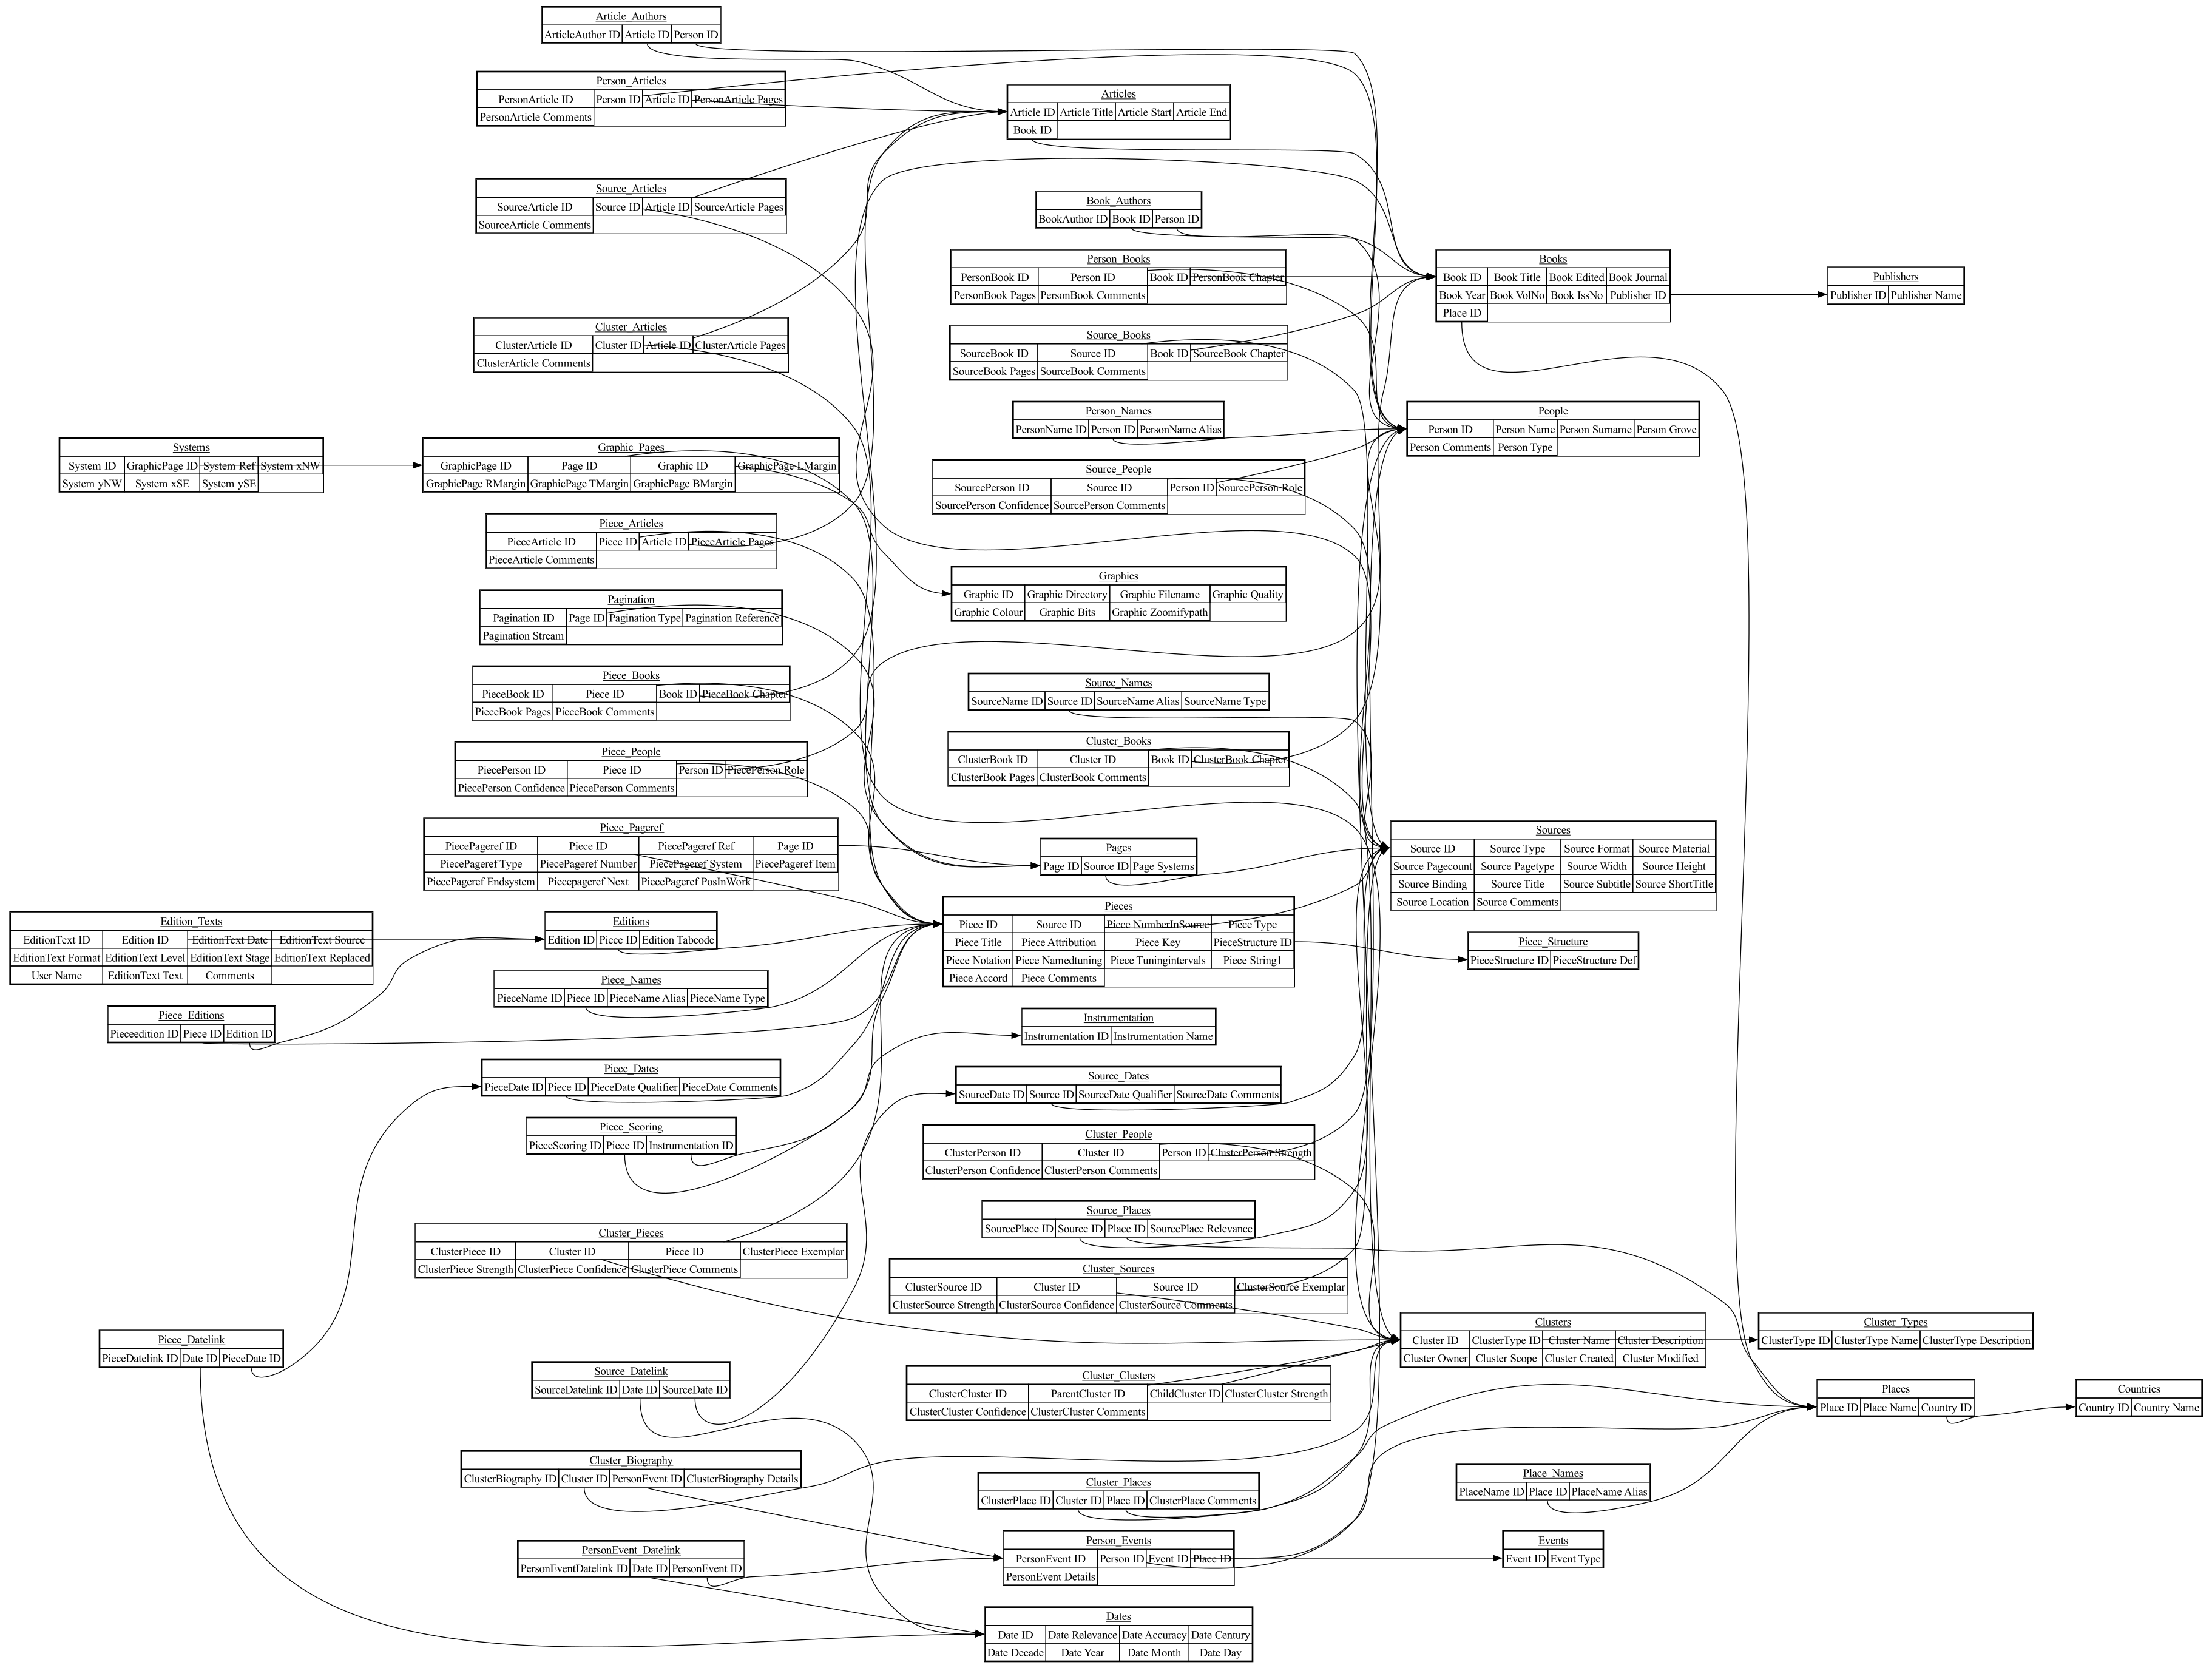
\includegraphics[width=\textwidth]{plot/records}
  \label{fig:records}
  \end{figure*}

  ECOLM I and II store all data directly in a relational database. The
  database contains both editorial tables, about users of ECOLM and
  their contributions, and record tables, about the works in the
  dataset. Figure \ref{fig:records} shows the record tables.

  The schema models join relationships using either foreign keys
  (e.g. {\tt Source ID} in {\tt Pieces}) or join tables (e.g. {\tt
    Person\_Events}) depending on the presence of metadata about the
  relationship.

  ECOLM has specific definitions of ``piece'' and ``work''. A piece is
  ``a single musical entity within a specified source'', while a work
  is ``a cluster of pieces in different sources that all represent the
  same musical work''. The database also uses ``cluster'' to record
  groups other than works. For example, the ECOLM II database contains
  only 9 ``pieces'' directly linked to John Dowland as composer or
  scribe, but 109 ``pieces'' linked to him through clusters: 105 as
  members of the Lachrimae ``group'' cluster, and 4 others through
  ``work'' clusters.

  The ECOLM schema is unusual today in using mixed-case naming with
  spaces in the column names.
  
  \clearpage

  \subsection{RISM Muscat web application}\label{muscat-data}
  
  \begin{figure*}[b]
  \centering
  \caption{RISM Muscat schema summary}
  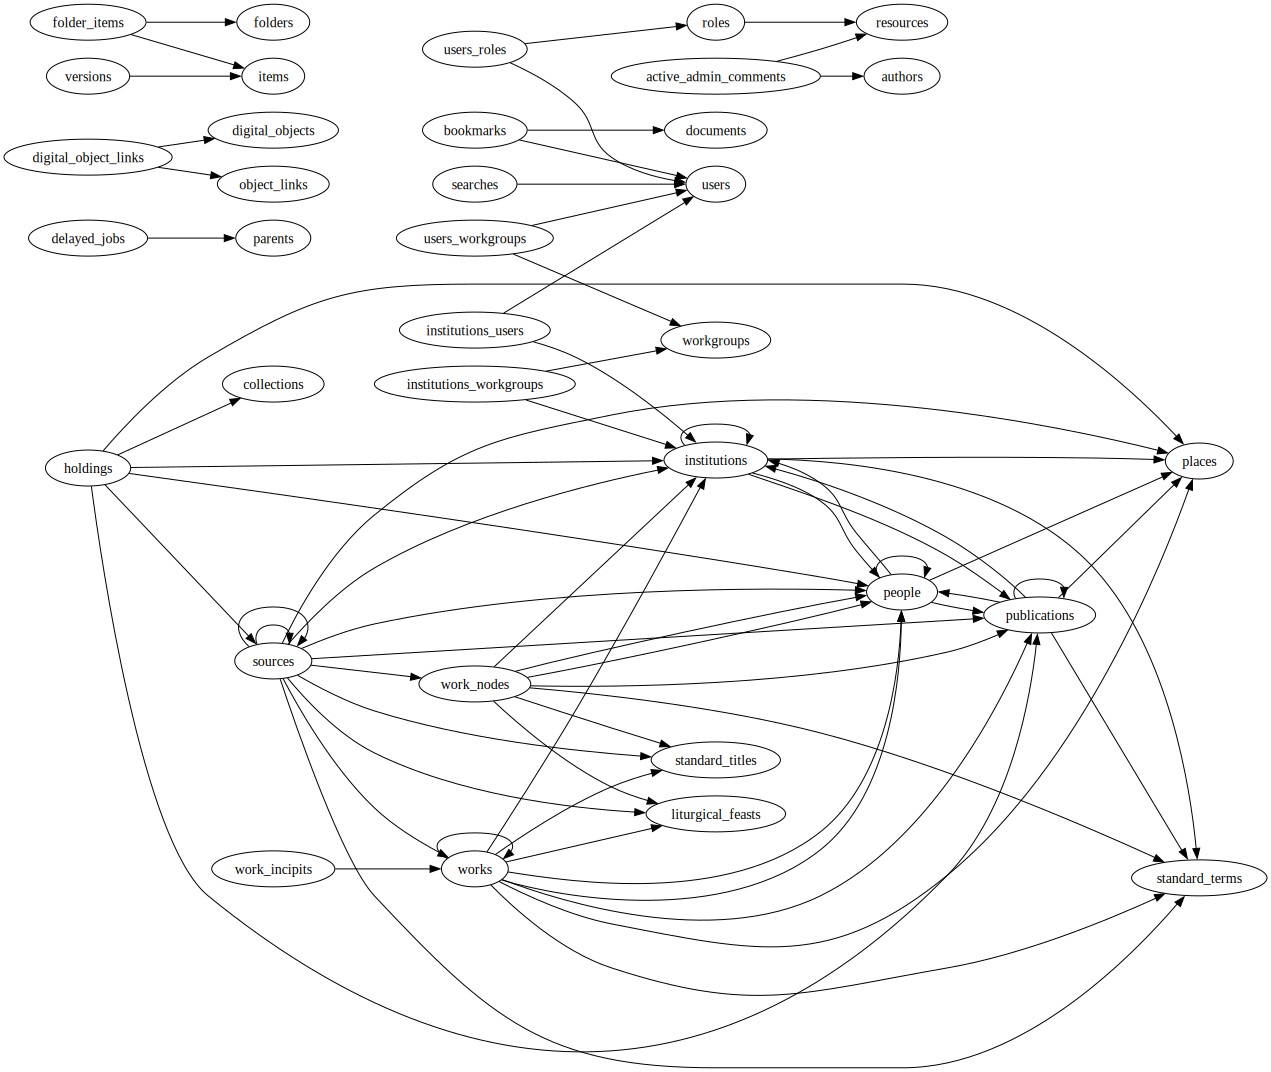
\includegraphics[width=\textwidth]{plot/muscat}
  \label{fig:muscat}
  \end{figure*}

  Muscat\footnote{https://rism.info/community/muscat.html} is a web
  application published by RISM for cataloguing musical sources,
  written using Ruby on Rails. Figure \ref{fig:muscat} shows the main
  tables.

  Muscat uses a hybrid schema, in that each table has a single {\tt
    marc\_source} column containing an authoritative record in
  MARC21\footnote{https://www.loc.gov/marc/} concise text format. Most
  of the other columns are apparently used to ``cache'' data from the
  MARC record that may be needed quickly for display or search. At
  core, everything is represented using MARC.

  Muscat also adds metadata, such as MARC tags, to joins (the arrows
  in figure \ref{fig:muscat}) through the use of separate join tables.
  
  As an example, the core {\tt sources} table contains columns for
  numerical RISM source ID, standardised title, manuscript title,
  composer, shelf mark, language, and date, along with downcased
  simplified versions of the composer and titles for search
  purposes. But the authoritative data is found in the {\tt
    marc\_source} column. There are no foreign key relations, as joins
  are managed through join tables such as {\tt sources\_to\_people},
  {\tt sources\_to\_sources} etc.
  
\end{sloppypar}
\end{document}
